\begin{frame}
    \frametitle{Ausweg: Koordinatentransformation}
    
    Gesucht wird ein Koordinatensystem, indem die kanonischen Gleichungen direkt gelöst werden können.
    
    \begin{figure}
        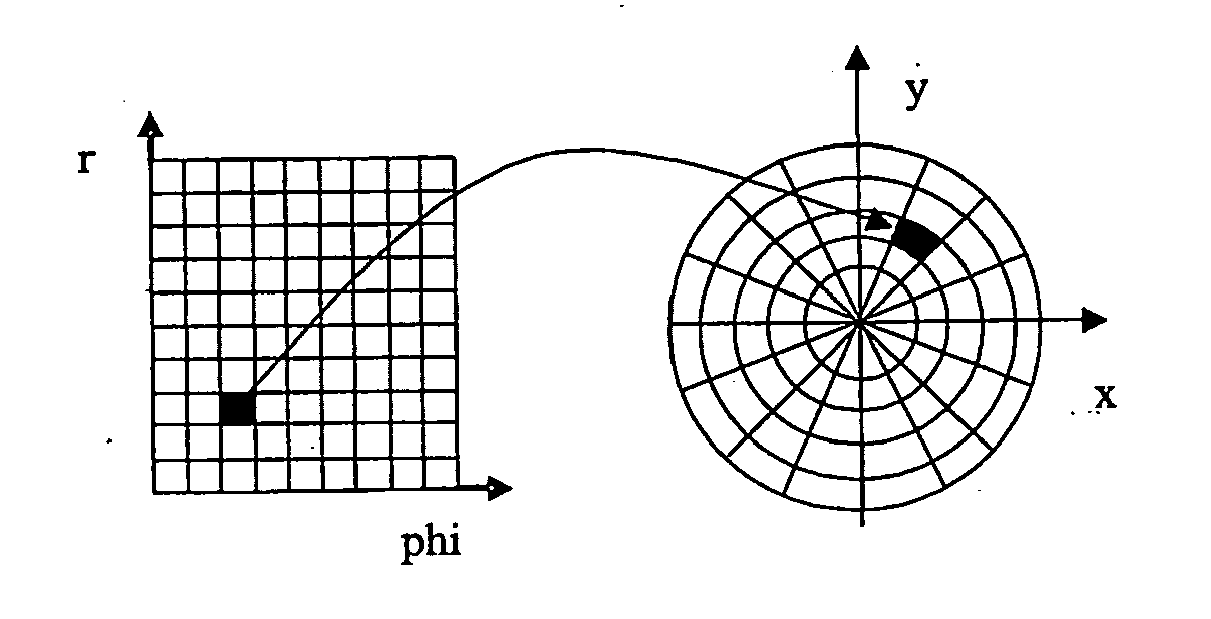
\includegraphics[scale=0.2]{images/koordtrans.png}
    \end{figure}
    
    
\end{frame}

\begin{frame}
    \frametitle{Ausweg: Koordinatentransformation}
    
    \textbf{Wichtig:} Lösungen müssen erhalten bleiben.\\
    D.h. wir brauchen Transformationen, gegenüber derer die kanonischen Gleichungen invariant sind. \\
    \vspace{5mm}    
    Solche Transformationen werden \emph{kanonische Transformationen} genannt.
    
    \begin{figure}
        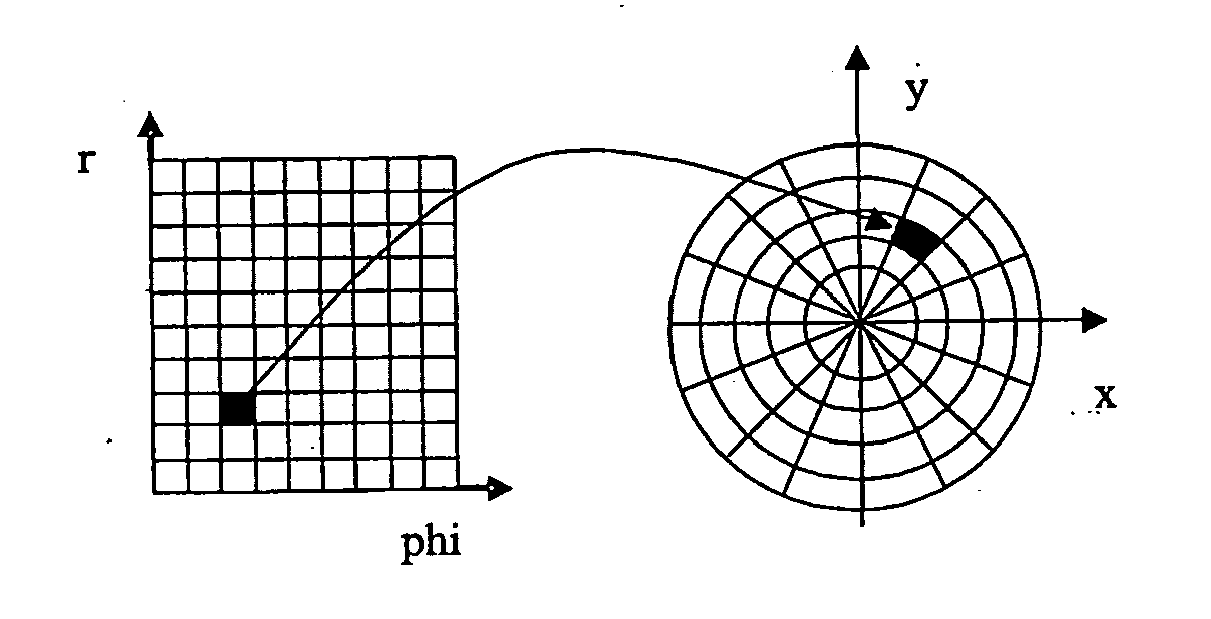
\includegraphics[scale=0.2]{images/koordtrans.png}
    \end{figure}
    
    
\end{frame}